\documentclass[oneside,final,14pt]{extreport}
\usepackage[utf8]{inputenc}
\usepackage[ukrainian]{babel}
\usepackage{vmargin}
\usepackage{graphicx}
\usepackage{float}
\usepackage{amsmath}
\usepackage{csquotes}
\usepackage{subfig}
\setpapersize{A4}
\setmarginsrb{2cm}{1.5cm}{1cm}{1.5cm}{0pt}{0mm}{0pt}{13mm}
\usepackage{indentfirst}
\sloppy
\begin{document}
\begin{large}
\begin{centering}
	\thispagestyle{empty}
НАЦІОНАЛЬНИЙ ТЕХНІЧНИЙ УНІВЕРСИТЕТ УКРАЇНИ \\
«КИЇВСЬКИЙ ПОЛІТЕХНІЧНИЙ ІНСТИТУТ» ІМЕНІ ІГОРЯ СІКОРСЬКОГО\\
ІНСТИТУТ ПРИКЛАДНОГО СИСТЕМНОГО АНАЛІЗУ\\
КАФЕДРА МАТЕМАТИЧНИХ МЕТОДІВ СИСТЕМНОГО АНАЛІЗУ\\
\vfill
{\bfseries "`Розробка програм аналізу та генерації псевдовипадкових чисел"'\\
ua}\\
Курсова робота\\
дисципліна\\
{\itshape "`Алгоритмізація та програмування"'}\\
\end{centering}
\vfill



\begin{flushright}
 Виконавець:\\
	Федурко Микола КА-75\\
Керівник:\\
Романов В. В.\\
\end{flushright}
\bigskip
\begin{flushleft}
“Захист дозволено”\\
“\_\_\_\_”\_\_\_\_\_\_\_\ 2018 р.\\
Захищено з оцінкою:\\
\vfill
\centerline{
Київ 2018}
\end{flushleft}
\newpage
\setcounter{page}{2}
\section*{Завдання}\label{s:0}
Розробити програму генерації псевдовипадкових чисел в залежності від вибраної 
функції розподілення з можливістю роботи з файлами (запис та зчитування функції),
 а також результатів генерації.
\tableofcontents

\chapter*{Вступ}\label{c:1}
\addcontentsline{toc}{chapter}{Вступ}
В еру розквіту комп'ютерних технологій, цей світ стає все більш визначеним. 
Скільки пройшло часу з зародження кібернетики як всесвітньо відомої науки, 
а знаходження незакономірних чисел до цих пір дуже потрібне в цій і багатьох 
інших галузях.

Задача знаходження випадкових чисел виникла в найнеочікуваніших областях 
кібернетики і прикладного програмного забезпечення. Починаючи з криптографії 
і закінчуючи використанням в лотереях.

Якщо вдуматися в рішення цієї задачі, то можна легко прийти до очевидного 
рішення - використовувати фізику для генерації випадкових значень. Можна 
використовувати шуми навколишнього середовища, або вологість повітря в тихому 
океані, як пропонують нам відомі ресурси генерації випадкових чисел.

Це рішення даної проблеми, не зовсім коректне, адже шуми і скачки вологості - 
цілком детерміновані(визначені) фізичні явища. З теоретичної точки зору 
знаючи початкові умови замкнутої системи можна визначити всі її подальші 
тани в будь-який момент часу. Для цього лише потрібна достатня потужність 
ЕОМ(Електронно-обчислювальної машини). Мусимо зауважити, що існує відносно 
молода сім'я теорій квантової фізики, яка стверджує, що явища 
мікросвіту(світу квантів) можна описувати лише за допомогою теорії ймовірності, 
тобто випадково. Але оскільки людство поки що не може впевнитися в цьому,
 ми опустимо цей варіант. 

Також можливі ситуації, коли використання фізики для вирішення задачі 
неможливе, або не вигідне. Мається на увазі обмеженість в ресурсах 
вбудовуваних систем. Адже, підключення додаткових пристроїв і завантаження 
коду в "<польових"> умовах не завжди можливе.

Отже приходимо до задачі створення програмних продуктів для генерації 
випадкових значень засобами математики. Що на перший погляд є не такою 
вже й складною задачею. Візьмемо наприклад число  яке за спостереженнями 
цілковито випадкове та нескінченне. Тут же приходимо до висновку, що щоб 
взяти випадкову цифру потрібно згенерувати випадковий номер цієї цифри, 
заходимо в замкнуте коло. 

Саме тому логічним кроком буде створення продукту для такої генерації 
засобами математичного апарату, щоб знаючи всі попередні значення 
згенерованих даних не мати можливості прогнозувати наступне, що і є 
метою даної роботи.

Для проекту була обрана мова програмування "<С">, саме через швидкість 
своєї роботи та лаконічний синтаксис.

\chapter{Обгрунтування і вибір алгоритмів}\label{c:2}
Прийшовши в попередньому розділі до необхідності створення програмного 
забезпечення, логічно описати ряд вимог, яким мусить задовольняти 
обраний алгоритм.

\section{Означення}\label{s:21}
Спочатку введемо деякі означення і скорочення:\\
ГПВЧ - генератор псевдовипадкових чисел, програмне забзепечення, 
що задовольняє умові непередбачуваності, детальніше описаній в 
останньому абзаці вступу. Відрізняється від ГВЧ(генератора випадкових чисел) 
цілковитою визначенністю.

Оскільки ми використовуємо математичний апарат, то цілковитої 
невизначенності не вийде досягнути. Дійсно, коли ми генеруємо послідовність, то  
кожен наступний член визначається попереднім, отже, чисто теоретично 
можлива ситуація коли послідовність почне зациклюватись з певним періодом. 
Далі буде показано, що це неминуча ситуація.

Період ГПВЧ - кількість елементів між першим входженням даного елемента 
і його другим входженням. 

Також потрібно все ж таки якимось чином задати початкове значення, 
адже в протилежному випадку всі значення будуть однакові.

Ключ ГПВЧ - початкове значення послідовності випадкових чисел. 
Також відомий як seed (англ. - зерно). 

\section{Вимоги}\label{s:22}
З уж~е чітко окресленою термінологією доцільно оголосити 
список вимог, яким мусить задовольняти наш алгоритм ГПВЧ:
\begin{itemize}
	\item 
Достатньо довгий період, що гарантує відсутність зациклювання 
в межах цієї задачі. Довжина періоду мусить бути математично-доведеною.
	\item 
Портабельність - дана реалізація мусить функціонувати на різних 
системах однаково.
	\item 
Відтворюваність - можливість відтворити дану послідовність 
довільну кількість разів. Це особливо важливо при проведенні 
різних статистичних дослідів, для можливості записати результати.
	\item 
Ефективність - швидкий час роботи алгоритму, та малі затрати 
за пам'яттю
	\item 
Швидкість отримання \(X_{n+i}\) елемента послідовності чисел за відомими 
Xnелементом для довільного i. Це дозволяє розділяти послідовність 
на декілька потоків(послідовностей).
	\item 
Також існують декілька тестів для перевірки послідовності на 
"<випадковість">, до таких відносяться:
	\item 
DIEHARD
	\item 
NIST
	\item 
Тести Дональда Кнута
	\item 
Тест на останній біт - один із тестів для перевірки 
ГПВЧ на криптостійкість(властивість алгоритму протистояти 
криптоаналізу). Сам тест звучить так: якщо не існує 
поліноміального(зі складністю \(O(n^k)\) алгоритму, який знаючи 
перші \(k\) біт послідовності зможе знайти \(k + 1\) біт з ймовірністю 
більше \(50\%\), то такий ГПВЧ не пройшов тесту.
\end{itemize}

Попри велику множину графічних, статистичних тестів, кількість яких
 все росте, в 1982 році китайський вчений Ендрю Ян довів \cite{b2}, що ГПВЧ, 
 який пройшов "<тест на останній біт"> пройде також і всі інші тести, 
 виконувані за поліноміальний час.

Зациклення будь-якої послідовності ПВЧ прийняте, як постулат в 
підрозділі (\ref{s:21}) мусить бути доведене.\\
Доведення:

	ГПВЧ, можна розглянути, як функцію \(f\) на множині \(X\) (формула \ref{f:21})
\begin{equation}
	f: X \mapsto X
	\label{f:21}
\end{equation}
	

З елементарних комбінаторних міркувань це відображення має 
скінченну кількість комбінацій. Тобто якою б великою множиною 
не було X, є на порядки більша (але, що важливо скінченна) кількість 
кроків, після яких буде відбуватись повтор. Що і необхідно було довести.

\section{Розгляд алгоритмів генерації псевдовипадкових чисел}\label{s:23}
Після постановки ряду вимог до наших алгоритмів, логічним продовженням
 буде розгляд декількох алгоритмів, та відбір з них тих, що найкраще 
 підходять під вище описані потреби. 

\subsection{Лінійний конгруентний метод}\label{ss:231}
Одним із простих і популярних методів на сьогодні є лінійний конгруентний 
метод (ЛКМ), запропонований Д. Г. Лехмером в 1949 році. В його основі 
лежить вибір чотирьох ключових чисел:
\begin{itemize}
\item	\(m > 0\), - модуль;
\item  \(0 \leq a \leq m\), - множник;
\item  \(0 \leq c \leq m\), - приріст (інкремент);
\item  \(0 \leq X_0 \leq m\), - початкове значення(seed); 
\end{itemize}

Послідовність ПВЧ, яка отримується формулою (\ref{f:22}) називається лінійною 
конгруентною послідовністю (ЛКП). Ключом(seed) для неї слугує \(X_0\).
\begin{equation}
X_{n + 1} = (a \cdot X_n + c)\:mod \: m,\:n \geq 1 
\label{f:22}
\end{equation}

В даній формулі надзвичайно важливий мудрий підбір параметрів. Наприклад при
\(X_0 = 7, a = 8, c = 9, m =10\) отримуємо послідовність  7, 5, 9, 7, 5, 9, 1, ...
Послідовність взагалі не виглядає випадковою. Переконливі і
 цікаві ілюстрації, до цих прикладів можна знайти у \cite{b1}.

Існує узагальнення формули ЛКМ:
\begin{equation}
	X_{n + 1} = (a^k \cdot X_n + \frac{a^k - 1}{a - 1} \cdot c) \:mod \:m,\: k \geq 0,\: n \geq 0
	\label{f:23}	
\end{equation}
Доцільно розглянути задачу правильного підбору параметрів.Не вдаючись в доведення, 
яке було проведено в \cite{b1} та \cite{b3}, можна стверджувати: 
\begin{itemize}
	\item мусить бути достатньо великим
	\item значення $m$ розумно вибирати рівним $2q$, де $q$ - число 
	бітів в машинному слові, оскільки це дозволяє не приміняти 
	ділення по модулю в формулі (\ref{f:23})	 
\end{itemize}

Теорема (2.1.) Лінійна конгруентна послідовність, визначена 
параметрами $m,\:a,\: c,\: X_0$, має період $m$ т. т. т. к.(тоді і тільки тоді, коли):
Числа $с$ і $m$ взаємно прості;
\begin{enumerate}
	\item $(a - 1) \: \vdots \: p$, для деякого простого $p$, яке є дільником $m$
	\item $(a - 1) \vdots \: 4$, якщо $m\: \vdots \: 4$
\end{enumerate}

Доведення даної теореми, було освітлено в \cite{b3}.
	Також, дізнатися про список "<вдалих"> констант для цього 
	методу та цікаві факти з його історії, можна в \cite{b4}.
Підводячи підсумки:

Переваги:
\begin{itemize}
	\item Простота реалізації
	\item Універсальність 
\end{itemize}Швидкість
Недоліки:
\begin{itemize}
	\item Простота "<взлому"> показана в \cite{b5} та \cite{b6}
\end{itemize}

Тим не менше ЛКМ, виявився доволі корисним, для не криптографічних 
задач, таких як моделювання та ігрові програми. Не дивлячись на його
 проблему, на сьогодні його використовують в таких мовах програмування, як Java, C, C++, C\#.

\subsection{Реєстр зсуву з лінійним зворотнім зв'язком. Метод М-послідовності}\label{ss:232}
Наступний клас ГПВЧ містить в основі ідею перетворення бітів деякого числа.
Реєстр зсуву - впорядкований набір бітів, допускаючий операцію зміни позиції 
цих бітів на одну й ту ж величину. 

Реєстр зсуву з лінійним зворотнім зв'язком (РЗЛЗЗ) - реєстр зсуву бітових слів,
 у якого вхідний біт, є лінійною функцією інших бітів. Вхідний біт стає в комірку 
 з номером нуль. Кількість комірок p називають довжиною реєстру.

 Для натурального числа p і a1,a2,... ,ap-1 ,  що приймають значення 0 або 1, 
	визначена рекурентна формула (\ref{f:24})
	\begin{equation}
	X_{n+p} = a_{p-1}X_{n+p-1}+a_{p-2}X_{n+p-2}+ \cdots +a_{1}X_{n+1}+X_n
	\label{f:24}
	\end{equation}

	Як видно з формули (\ref{f:4}), для РЗЛЗЗ функція зворотнього зв`язку є лінійною
	 булевою функцією, залежною від стану всіх чи декотрих бітів реєстру.

	 Одна ітерація алгоритму, який генерує послідовність, складається з наступних кроків:
\begin{enumerate}
	\item 
Зміст комірки p - 1 формує формує черговий біт ПСП бітів.
	\item
Зміст комірки 0 визначається значенням функції, обчислюваним за формулою (\ref{f:24}).
	\item
Зміст кожного \(і\)-го біта переміщується в \((i+1)\)-й, \(0 \leq i<p-1\).
	\item
В комірку 0 записується значення з кроку 2.
\end{enumerate}

	Найбільше додатнє значення \(N\) таке, що \(X_{n + N}=X_n \forall n\)називають періодом 
	послідовності. Цю послідовність називають \(M\)-послідовністю, якщо її період 
	рівний \((2p-1)\). Буква "<\(M\)"> в назві від англійського "<maximum">. Дійсно, адже 
	максимальний можливий період і є періодом цієї послідовності. 
	На рис. \ref{p:1} зображено алгоритм роботи даного ГПВЧ для формули (\ref{f:24}), де \(F(x)\) ---
	лінійна функція зворотнього зв'язку:
	\begin{figure}[H]
		\centering
		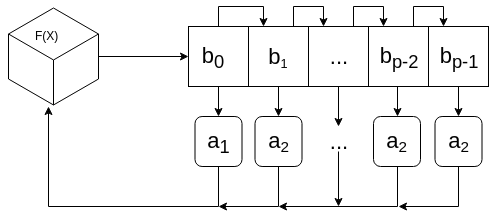
\includegraphics[width=0.5\textwidth]{rzlzz.png}
		\caption{Схема роботи РЗЛЗЗ}
		\label{p:1}
	\end{figure}
Визначимо, які вхідні дані відповідають \(M\)-послідовності(з найбільшим періодом), для цього введемо означення:

Многочлен \(F(x)\) степені \(p\) називається примітивним, якщо він не ділить націло многочлен  виду \((x^s-1)\),  
де \(s < 2^p-1\).

Найменше натуральне число \(e\) при якому \(x^e-1 \: \vdots \: F(x)\) називається показником многочлена.

Властивості послідовності бітів залежать від многочлена (\ref{f:24})
\begin{itemize}
	\item
Якщо старший коефіцієнт \(a_p=0\), то періодичність згенерованої послідовності може проявитися не одразу.
	\item 
Якщо старший коефіцієнт \(a_p=1\), то послідовність буде періодичною з самого початку
	\item
Якщо \(k = 1\), то примітивність многочлена (\ref{f:24}) є необхідною і достатньою умовою того, 
що ПСП згенерована РЗЛЗЗ буде мати максимальну довжину \(N = 2^{p-1}\).
\end{itemize}

Підсумовуючи:

Переваги:
\begin{itemize}
	\item 
Швидкість
	\item
"<Хороші"> статистичні властивості
	\item
Простота реалізації на програмному рівні
\end{itemize}

Недоліки:
\begin{itemize}
	\item
Повільна програмна реалізація
	\item
Можливість взлому за \cite{b7} та \cite{b8}
	\item
РЗЛЗЗ використовуються у вбудовуваних системах, саме через простоту апаратної реалізації.
\end{itemize}
\subsection{Вихор Мерсенна}\label{ss:233}

Метод Вихор Мерсенна був запропонований в 1997 році японськими вченими Макото Мацумото 
та Такудзі Нісімура. Введемо деякі означення:
"<Вихор"> - перетворення, що забезпечує рівномірний розподіл ПВЧ.
Число Мерсенна - натуральне число Mn, визначене формулою (\ref{f:25}):
\begin{equation}
	M_n=2^n-1
	\label{f:25}
\end{equation} 

Однією із важливих властивостей цих чисел є те, що якщо Mn просте, то n - також просте. 
Є багато варіацій цього алгоритму, розглянемо MT19937 - найпопулярніший варіант. По суті, 
даний ГПВЧ є  РЗЛЗЗ, який складається з 624 комірок по 32 біта, та генерується за формулою (\ref{f:26}):
\begin{equation}
X_{n+p}=X_{n+q} \bigoplus (X_n^r | X_{n+1}^l) A     \;\;      (n = 0,1,2,...)
\label{f:26}
\end{equation}

Де
\begin{itemize}
	\item
\(p, q, r\) --- цілі константи, \(p\) --- степінь рекурентності, \(1 \leq q \leq p\);
	\item
$X_n$ --- w-бітне двійкове число
	\item 
$(X_{n}^r | X_{n+1}^l)$ - двійкове ціле число, отримане конкатенацією(об'єднанням) чисел 
	\item
$X_n^r$ та $X_{n+1}^l$, де перші $(w-r)$ бітів отримані із $X_n$, а останні $r$ бітів із $X_{n+1}$
	\item
A - матриця нулів і одиниць порядка w, визначена за допомогою формули (\ref{f:27}).
	\item
$XA$ - добуток, при обчисленні якого спочатку виконують операцію $X \gg 1$(зсув на один вправо), 
якщо останній біт дорівнює 0, потім коли останній біт дорівнює 1, обчислюється $XA = (X \gg 1)a$.
\end{itemize}
\begin{equation}
	\begin{split}
	a &= (a_{w-1}, a_{w-2}, \cdots, a_0) \\
	X &= (x_{w-1}, x_{w-2}, \cdots, x_0) \\
	\label{f:27}
	\end{split}
\end{equation}
\\\\
\[
	\left(
		\begin{matrix}
			0 & 1 & 0 & \cdots & \cdots & 0 \\
			0 & 0 & 1 & \cdots & \cdots & 0 \\
			0 & 0 & 0 &  &  & 0 \\
			\vdots & \cdots &  & \ddots &  & \vdots \\
			0 & 0 & \cdots &  & \ddots & 1 \\
			a_{w-1} & a_{w-2} & \cdots & \cdots &  & a_0 \\
		\end{matrix}
	\right)
\]
\\

Кроки виконання алгоритму Мерсенна:
\begin{enumerate}
	\item\label{step:21} Ініціалізація значень $u$, $h$, $a$ за формулами (\ref{f:28})
	\begin{equation}
		\begin{split}
	u &= (1, 0, \cdots,0) \textnormal{---} \; \textnormal{всього} \; (w-r) \; \textnormal{біт.}\\
	h &= (0, 1, \cdots ,1) \textnormal{---} \; \textnormal{всього} \; r \; \textnormal{біт}.               \\
	a &= (a_{w-1}, a_{w-2}, \cdots, a_0) \; \textnormal{--- остання строка матриці} \; A\\
		\end{split}
	\label{f:28}
	\end{equation}
	\item\label{step:22} Ініціалізація $X_0,X_1, \cdots, X_{p-1}$ 
	\item\label{step:23}
	\begin{equation} 
		Y=(y_0, y_1, \cdots, y_{w-1})
		\label{f:29}
	\end{equation},
	\item\label{step:24} Обчислення нового значення $X_i$:
	\begin{equation}
		\begin{split}
		X_n &= X_{(n+q)  \; mod \;  p} \bigoplus (Y \gg 1) \bigoplus a, \; \textnormal{якщо найменший біт} \; y_0=1;\\
		X_n &= X_{(n+q)  \; mod \;  p} \bigoplus (Y \gg 1) \bigoplus 0, \; \textnormal{якщо найменший біт} \; y_0=0;\\
		\end{split}
	\label{f:29}
	\end{equation}
	\item\label{step:25}
	Обчислення $X_j T$:
	\begin{equation}
		\begin{split}
		Y &= X_n;\\
		Y &= Y \bigoplus (Y \gg u);\\
		Y &=Y \bigoplus ((Y \ll s) \cdot b);\\
		Y &=Y \bigoplus ((Y \ll t) \cdot c);\\
		Z &=Y \bigoplus (Y \ll l).\\
		\end{split}
	\label{f:210}
	\end{equation}
	Z подається на вихід як результат.
	\item\label{step:26} $n = (n+1)  \; mod \;  p$, переходимо на крок \ref{step:23}
		Параметри алгоритму, ще з початку підібрані авторами, щоб давати найкращі 
		результати. $w$ обирається за розміром машинного слова, тому для 64-бітної версії 
		формула має інший вигляд.
		Параметри методу Вихор Мерсенна:
	\begin{displaymath}
		\begin{split}
		p &= 624,\; w = 32,\; r = 31,\; q = 397,\; \\
		a &= 2567483615(9908B0DF16),\; u = 11,\; \\
		s &= 7,\; t = 15,\; l =18\,\; b = 2636928640(9D2C568016),\\
		\; c &= 4022730752(EFC6000016) \\
		\end{split}
	\end{displaymath}. 	
	
\end{enumerate}
\newpage
Підсумовуючи:

Переваги:
\begin{itemize}
	\item Вже відкорельовані параметри, для "<хорошого"> результату
	\item Великий період, а саме $(2^{19937}-1)$
	\item Хороший статистичний розподіл
	\item Швидший за інші алгоритми
	
\end{itemize}

Недоліки:
\begin{itemize}
	\item Складність аналізу
	\item Складність реалізації
\end{itemize}

Мусимо зауважити, що цей же алгоритм використовується в ГПВЧ мови програмування PHP. 
Також є багато його варіацій з нахилом на різні параметри, такі як TinyMT(пам'ять), CryptMT(криптостійкість).

\section{Вибір алгоритмів та конкретизація ПЗ}\label{s:24}

Більшість інших видів генераторів можна переглянути в додатку 1. В основному це різноманітні 
комбінації двох вище описаних методів(РЗЛЗЗ і ЛК). Оскільки РЗЛЗЗ і лінійні конгруенті генератори 
формують деякий "<базис"> ГПВЧ, то доцільно розглянути саме їх, як приклад в цій роботі. Оскільки 
РЗЛЗЗ існує також багато видів, то зупинимося на найбільш практичному - Вихрові Мерсенна. А лінійний 
конгруентний генератор оберемо звичайним, оскільки це буде яскравим простим прикладом свого класу генераторів.

Потрібно буде зробити функції для генерації чисел в обох ГПВЧ. Для ЛК зробимо функцію, яка буде т
естувати параметри A, C, M формули (\ref{f:22}). Також для лінійного конгруентного метода розробимо функцію,
що буде "<ламати"> генератор, тобто отримувати множину всіх можливих значень A, C, M. Можна було б 
розробити такі ж функції і для МТ, але цей генератор уже збалансований на великий період і 
всі його змінні заздалегідь відомі, тобто все що треба зробити для його "<зламу"> - це реверсувати 
дії "<загартовування">, а саме крок \ref{step:26} в пункті \ref{ss:233}   

Також доцільно буде написати деякі допоміжні функції. Вони описані в наступному розділі(пункт \ref{s:31}), 
разом зі структурами та алгоритмами для рішення поставлених задач.
\chapter{Розробка програми}\label{c:3} 
Після надання теоретичних відомостей та обрання алгоритмів, логічно приступити до 
розробки алгоритмів та створення продукту.
\section{Опис допоміжних функцій}\label{s:31}
Оскільки функції, які ми обрали в пункті \ref{s:24} потребують "<допоміжних"> функцій, 
то доцільно спочатку описати останні, адже при опису процесу розробки основних функцій, ми 
будемо посилатися на цей розділ. Чесно кажучи процес розробки проходить навпаки, спочатку 
пишеться код, а потім, за необхідності, додаються функції, щоб структурувати цей код. 
Отже, в цьому пункті ми дамо алгоритми роботи цих функцій, але їхнє призначення
 буде розкрито в наступних пунктах.
\subsection{Генератор фізично-випадкових чисел}\label{ss:311}
{\bfseries
int getAbsStartRand();}\\
	Функція яка повертає випадкові числа. Для цього, якщо програма на unix-подібних системах, 
	то вона повертає значення папки "</dev/urandom">, яка чиатється, як прилад та містить 
	"<шуми"> комп'ютера у вигляді байтів. Якщо ж використовується Windows, то викликається 
	схожа функція під Windows. Таким чином створюються абсолютно випадкові значення. Якщо ж 
	відповідна функція повернула код помилки, то ми просто повертаємо {\itshape clock()} - час від початку 
	роботи програми, який уже є менш випадковим значенням.  

\subsection{Інші функції}\label{ss:312}
	Дамо перелік "<простих"> функцій, що також використовуються в більш складніших:
	\begin{itemize}
		\item 
		НСД - найбільший спільний дільник
		\item
		НСК - найбільше спільне кратне
		\item
		MOD - повертає завжди додатнє значення остачі від ділення числа на число
		\item
		Перевірка на простоту числа
		\item
		Знаходження максимального числа серед чотирьох чисел
	\end{itemize}

Всі оголошення описаних вище функцій помістимо в заголовковий файл {\itshape RandomFunctions.h}. 
А їх код помістимо в файл {\itshape RandomFunctions.c}. Див. додаток 2. Для цієї частини програми нам 
потрібні такі заголовкові файли:
\begin{itemize}
	\item 
	{\itshape stdlib.h} - бібліотека стандартних функції "<C">
	\item 
	{\itshape math.h} - функція для роботи з математикою
	\item 
	{\itshape time.h} - функція для роботи з часом (функція {\itshape clock()})
	\item 
	{\itshape inttypes.h} - додає деякі типи та специфікатори цих типів до функції {\itshape printf()}
	\item 
	{\itshape sys/random.h, fcntl.h, unistd.h} - для виклику {\itshape getrandom(...)}, лише для роботи під Unix
	\item 
	{\itshape Wincrypt.h} - для виклику {\itshape CryptGenRandom(...)}, лише для роботи під Windows 
\end{itemize}

\section{Реалізація методу "<Вихор Мерсенна">}\label{s:32}
	Частина програми, що відповідає за роботу Вихру Мерсенна складається з двох файлів: 
	{\itshape BIZ\_MT.c}, та {\itshape BIZ\_MT.h}. В другому розміщені оголошення функцій, макросів, 
	структур, а в першому самі функції.
\subsection{Структура MTRand}\label{ss:321}
Згідно з пунктом \ref{ss:233} створена структура MTRand, що зберігає значення констант 
і змінних для генерації чисел. Вона складається з таких полів:
\begin{itemize}
\item
{\itshape int32\_t *newx} --- масив для нової генерації значень
\item
{\itshape unsigned int arr\_len}  ---  $P$ (в позначеннях пункту \ref{ss:233})
\item
{\itshape unsigned int offset} ---  $Q$ (в позначках пункту \ref{ss:233})
\item
{\itshape unsigned int hardening0} --- $U$ (в позначках пункту \ref{ss:233})
\item
{\itshape unsigned int hardening1} --- $S$ (в позначках пункту \ref{ss:233})
\item
{\itshape int32\_t hardening2} --- $B$ (в позначках пункту \ref{ss:233})
\item
{\itshape unsigned int hardening3} --- $T$ (в позначках пункту \ref{ss:233})
\item
{\itshape int32\_t hardening4} --- $C$ (в позначках пункту \ref{ss:233})
\item
{\itshape unsigned int hardening5} --- $L$ (в позначках пункту \ref{ss:233})
\item
{\itshape int32\_t * x} --- масив початкових значень для генерації
\item
{\itshape int32\_t lower\_mask} --- $h$ (в позначках пункту \ref{ss:233})
\item
{\itshape int32\_t higher\_mask} --- $u$ (в позначках пункту \ref{ss:233})
\item
{\itshape int32\_t matrix\_row} --- $A$ (в позначках пункту \ref{ss:233})
\end{itemize}
Існує глобальний екземпляр цієї структури {\itshape MTRand mt\_def}, над яким 
і будуть відбуватись зміни, що дуже схоже на "<машину станів">, 
яка використовується наприклад в OpenGL.
\subsection{Функції ініціалізації використання та видалення генератора}\label{ss:322}
{\bfseries MTUserArray * mtRandInit(MTRand * rand);} \\

Функція яка ініціалізує структуру {\itshape mt\_def} початковими значеннями. 
Їй передається вказівник на структуру {\itshape rand}, якщо він дорівнює нулю, 
то {\itshape mt\_def} --- ініціалізується значеннями "<за замовчуванням">(описані вище константи). 
Потім виділяється пам'ять для масиву {\itshape mt\_def->newX} і {\itshape mt\_def->X}. 
Другий заповнюється початковими випадковими значеннями за допомогою функції 
{\itshape getAbsStartRand()} описаної в пункті \ref{ss:311}. 

Якщо ж користувач передає вказівник на свою структуру {\itshape MTRand * rand}, то всі значення 
ініціалізуються користувацькими даними. Якщо користувач передав свою структуру, 
то логічно подумати, що у нього є свої початкові значення, тобто пам'ять виділяється 
лише під масив {\itshape rand->newX}, при чому вказівник {\itshape mt\_def->newX} вказує на ту ж область пам'яті, 
для того щоб спокійно працювати з нею і надалі. Адже всі взаємодії здійснюються за допомогою {\itshape mt\_def}. 

Далі створюється вказівник на структуру {\itshape MTUserArray * MTArr}, під який виділяється 
пам'ять та поля якого заповнюються відповідно: 
\begin{itemize}
\item
{\itshape MTArr->ptr = \itshape mt\_def.newX;}
\item 
{\itshape MTArr->len = mt\_def.arr\_len;}
\end{itemize}

Ця структура повертається, це зроблено для зручної роботи користувача, адже таким 
чином він має доступ до згенерованих значень. Мусимо зауважити, що в функцію передається 
саме вказівник, щоб надати можливість обрати режим "<за замовчуванням">.

{\bfseries void mtDefRand()};\\
	Оскільки генерація відбувається крок в крок за алгоритмом описаним в пункті \ref{ss:233}, 
	то немає ані найменшого сенсу повторюватися. Проте звертаємо увагу, на те, що нове значення 
	записується шляхом математичних дій над {\itshape mt\_def->x} та записується в {\itshape mt\_def->newX}. 
	Тому, щоб повторити цикл, користувачу необхідно викликати функцію {\itshape void mtDefSwapBuffers();}

{\bfseries void mtDefKill(MTUserArray * MTArr);}\\
	На момент видалення у користувача є структура із згенерованими значеннями, 
	пам'ять для якої була виділена динамічно, тобто її потрібно вивільнити(принаймні в "<С">). 
	Він передає вказівник, а ми очищаємо пам'ять під нього, також вивільняючи пам'ять 
	масивів {\itshape mt\_def->x}, {\itshape mt\_def->newX}.
\section{Реалізація лінійного конгруентного генератора}\label{s:33}
Частина програми, що відповідає за роботу лінійного конгруентного генератора складається 
з двох файлів: {\itshape BIZ\_LKM.c}, та {\itshape BIZ\_LKM.h}. В другому розміщені оголошення функцій, макросів,
 структур, а в першому самі функції. 
\subsection{Структури мови "<С"> використані при реалізації}\label{ss:331}
 {\bfseries struct LKMSet;}\\
Має три поля: $a,\; c,\; m$. Використовується для зберігання пар ${A, \;C,\; M}$ формули (\ref{f:22}). Надалі для 
більшості змінних цієї частини програми використовуються тип "<int64\_t"> заголовкового файлу 
"<inttypes.h">. В заголовковому файлі уже є 15 варіантів "<хорошого"> вибору параметрів, тобто 
їх можна використовувати у своїх програмах.

{\bfseries struct LKMUserArray;}

{\bfseries void free\_array(LKMUserArray ** arr);}

	Має два поля: {\itshape len, set}. {\itshape set} - вказівник(в перспективі - массив) структур {\itshape LKMSet}. 
	{\itshape len} ---
	довжина цього масиву. Використовується для взаємодії користувача з функціями "<зламу"> 
	генератора. Оскільки в основному в програмі будуть використані вказівники на цю структуру, 
	то єдина незначна функція цього пункту відповідає за очищення динамічно виділеної пам'яті під цю структуру.

{\bfseries struct LKMRand;}\\
	Має два поля: {\itshape seed, set}. {\itshape set} --- структура описана в першому абзаці. 
	{\itshape seed} - початкове значення для генератора. Тобто ця структура є користувацьким 
	генератором, який він може протестувати, привести в дію, зламати. В заголовковому 
	файлі "<за замовчуванням"> оголошений екземпляр цієї структури {\itshape lkm\_def}, який(як описано 
	на сторінці \pageref{ss:321}) створює абстракцію машини станів.
\subsection{Функція ініціалізації і використання генератора}\label{ss:332}
{\bfseries void lkmRandInit(LKMrand * rand);}

	{\itshape rand} --- користувацькі параметри, згруповані в структуру. Коли користувач передає 
	вказівник на структуру, то структура {\itshape mt\_def} приймає свої значення за наступними правилами:
Початкове значення({\itshape lkm\_def.seed}) присвоюється остача від ділення користувацького 
початкового значення({\itshape rand->seed}) на {\itshape rand->set.m}. Що зроблено для профілактики помилок, 
коли користувач задасть початковим значенням число більше {\itshape rand->set.m}.
Те ж відбувається і з параметрами {\itshape lkm\_def.set.a, lkm\_def.set.c}.
Значення {\itshape rand->set.m} присвоюється {\itshape lkm\_def.set.m}
	Якщо ж користувач передасть в функцію {\itshape NULL}, то всі параметри {\itshape lkm\_def} заповняться 
	константами "<за замовчуванням">. Окрім {\itshape seed}`a який буде отриманий за допомогою нашого 
	генератора випадкових чисел, опис якого наданий в пункті \ref{ss:311}. Ще раз наголосимо, що 
	в функцію передається вказівник для можливості реалізації значення 
	"<за замовчуванням">(детальніше описано в останньому абзаці пункта \ref{ss:322}).

{\bfseries int64\_t lkmDefRand();}\\
	Функція генерації чітко описується формулою (\ref{f:22}). Нове значення присвюється 
	{\itshape lkm\_def.seed} і повертається.
\subsection{Опис функції аналізу обраних параметрів}\label{ss:333}
{\bfseries void lkmTestParam(LKMSet * set);}\\
	Функція яка отримує на вхід набір значень, обробляє його і дає корисні поради для покращення 
	результатів. Під "<результатами"> мається на увазі довжина періоду згенерованих значень.
	Для обробки вона керується принципами описаними в пункті \ref{ss:231}. Виводить всі зауваження, 
	якщо таких немає, то хвалить користувача за вдалий вибір. Якщо такі все ж були, то вона 
	пропонує обрати з можливих "<хороших"> значень описаних в заголовковому файлі. Якщо ж користувач 
	і цього не хоче, то вона пропонує ввести нові значення самостійно. В разі обрання нових значень 
	вона запускає себе ще раз через {\itshape goto START}. В протилежному випадку функція закінчує свою дію. 

	Є неабияке бажання наголосити, що оператор переходу "<goto"> використовується для лаконічності і 
зрозумілості коду, оскільки:
\begin{itemize}
	\item
Використовувати ще один зовнішній цикл і змінні для керуванням користувацьким рішенням дуже погано 
впливає на читабельність коду
\item
Використання рекурсії призведе до неясності у виводі програми, оскільки після завершення всіх функцій, 
вони будуть декілька раз виводити результати своєї роботи, та і взагалі рекурсія - ресурсозатратна річ, 
оскільки вимагає заміну стека.
\end{itemize}

{\itshape START} - дуже зрозуміле ім'я для переходу
\subsection{Опис функції "<зламу"> генератора}\label{ss:334}
{\bfseries void lkmCrack(LKMUserArray ** arr, int64\_t x0,  int64\_t x1,  int64\_t x2, int64\_t x3);}\\
Функція приймає на вхід користувацький масив для запису в нього списку можливих параметрів. 
Та чотирьох чисел, уявлення про які краще отримати із системи (\ref{f:31})
\begin{equation}
	\begin{cases} 
	X_1 & = (A*X_0+C) \; mod \; M;\\
	X_2 & = (A*X_1+C) \; mod \; M; \\ 
	X_3 & = (A*X_2+C) \; mod \; M; 
	\end{cases}
	\label{f:31}
\end{equation}

У нас є три невідомі змінні $A, \;C, \;M,$ які будуть записані в 
{\itshape (*arr)->set[i]}. Де $i$ - деяке ціле число, яке залежить від кількості 
можливих варіантів цього генератора.

Алгоритм роботи цієї функції чітко описаний в \cite{b9}, тому немає сенсу 
	описувати його тут, також його опис може бути легко зрозумілий дивлячись '
	на коментарі до коду в додатку 2.
\subsection{Опис функції зменшення списку можливих варіантів}\label{ss:335}
{\bfseries void lkmRedList(LKMUserArray ** arr);}\\

Оскільки після роботи функції з попереднього пункту ми отримали масив 
	можливих варіантів параметрів, то логічно, що вибагливий користувач може
	 бути не задоволений кількістю варіантів, які треба перебрати. Хоча 
	 риптоаналітики будуть раді і цій інформації.
	 Саме тому було прийняте рішення написати ще одну функцію, яка буде зменшувати 
	(з англ. reduce) кількість можливих рішень "<зламу"> генератора. 

	Суть її полягає в тому, що вона запрошує дані для "<тестування">(формула (\ref{f:22})) 
	і перевіряє кожну трійку параметрів зі списку на відповідність цим даним. Під даними 
	мається на увазі X-и послідовності згенерованих чисел. 
	
	Якщо вони не відповідають, то 
	значення $m$ відповідного номеру зі списку встановлюється в $-1$. Оскільки множина роботи 
	функції з формули (\ref{f:22}) --- натуральні числа, то $-1$ --- чудовий виборі для попередження 
	про "<невідповідність"> конкретної трійки шуканому генератору.

	Якщо кількість "<відповідних"> варіантів зменшилось до нуля, то десь була допущена 
	помилка і програма повідомить вам про це.
	
	Якщо залишився лише один "<відповідний"> варіант, то програма привітає вас з успішним 
	"<зламом"> вашого генератора і завершить роботу.

\chapter{Керівництво користувачу}\label{c:4}

При користуванні функціями створеного ПЗ, потрібно керуватись наступними правилами:
\begin{enumerate}
	\item
Вводити значення тих типів, яких в тому чи іншому випадку потребує програма.
\item 
Надавати програмі реальних значень змінних, оскільки при наданні некоректних 
хідних даних програма, в більшості випадків, буде повертати неправильні вихідні дані
\item
Краще прислухатися до порад аналізатора вхідних даних
\end{enumerate}

Оскільки даний програмний продукт створений, як основа для розробки подальших програм,
то керівництво користувачу логічно обмежується цими правилами. Проте написання користувацьких 
програм полягає на плечі розробника, який в свою чергу мусить написати "<Керівництво користувачу"> 
своєї програми.
\chapter{Керівництво розробнику}\label{c:5}
	Оскільки програма складається з декількох модулів, то їх необхідно підключити, 
	а саме підключити такі заголовкові файли:
	\begin{itemize}
\item RandomFunctions.h
\item BIZ\_MT.h
\item BIZ\_LKM.h
	\end{itemize}
Також при компіляції потрібно додати їх у свій проект, якщо ви працюєте в IDE, або компілювати в gcc з такою командою: 
\begin{verbatim}
	gcc -g Gen/BIZ\_LKM/BIZ\_LKM.c Gen/BIZ\_MT/BIZ\_MT.c 
					Gen/RandomFunctions.c your\_prog.c  -o your\_prog -lm	
\end{verbatim}

де {\itshape Gen} - папка в якій зберігаються файли, {\itshape your\_prog.c} --- файл коду вашої програми
У {\itshape МТ} і {\itshape LKM} є {\itshape makefile}, змісти яких такі:
\begin{itemize}
	\item
MT:\\
\begin{verbatim}
mt: BIZ\_MT.c ../RandomFunctions.c
	gcc -g BIZ\_MT.c ../RandomFunctions.c -o mt -lm	
\end{verbatim}

	\item
LKM:\\	
\begin{verbatim}
lkm: BIZ\_LKM.c ../RandomFunctions.c
	gcc -g BIZ\_LKM.c ../RandomFunctions.c -o lkm -lm	
\end{verbatim}
\end{itemize}
Наглядно файлове розміщення показане на рис. \ref{p:51}
\begin{figure}[H]
	\centering
	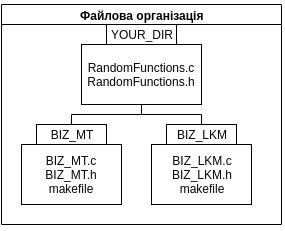
\includegraphics[width=0.6\textwidth]{proc.png}
	\caption{}
	\label{p:51}
\end{figure}
При роботі з функціями генераторів і допоміжними функціями доцільно перечитати розділ \ref{c:3}, 
в якому все детально описано. 
\chapter{Отримані результати}\label{c:6}
\section{Особливості трансляції, компонування і налагодження}\label{s:61}
	Програма написана на мові програмування "<С"> і компілювалася за 
	допомогою {\itshape gcc(GNU Compiler Collection)} в операційній системі {\itshape Manjaro} 
	{\itshape x86\_64}(в основі стоїть {\itshape Arch Linux}).
	Налагодження відбувалося за допомогою {\itshape gdb(GNU Debugger)}. Також була 
	використане інструментальне програмне забезпечення --- valgrind, для пошуку 
	витоків пам'яті при динамічному виділенні останньої.
	
	Мусимо зауважити, що програма працює крос-платформенно, 
	оскільки були використані функції із стандартної бібліотеки. І єдина 
	платформно-залежна функція {\itshape int getAbsStartRand();} була перероблена на незалежну, 
	шляхом розмежування її дій на кожній із систем.
\section{Результати рахунку контрольного прикладу}\label{s:62}
Нижче представлені десять із 624 значень функції {\itshape getAbsStartRand()} поданих 
на вхід алгоритму {\itshape MT19937}: \\
\begin{table}[H]
	\centering
\begin{tabular}{|c|c|c|c|c|}
	\hline 247985497  & 580701539 &  1529392703 &  912531385 &  1265435855 \\ \hline 
	 1302975498  & 1287154760  & 743203497 &  1768934035 &  334814459 \\ \hline
\end{tabular}
\caption{}
\label{t:62}
\end{table}


А результати роботи цього алгоритму представлені в таблиці(\ref{t:61}):\\
\begin{table}[H]
	\centering
\begin{tabular}{|c|c|c|c|c|}
	\hline
1071570338  & 1230189442 &  1995407069  & 1859497223 &  691350141 \\ \hline   
1025630334  &  662585518   &  742414615   &  257092565  &  1622530717 \\ \hline
\end{tabular}
\caption{}
\label{t:61}
\end{table}
Вхідне число та результати генерації 10 значень алгоритму ЛКМ представлені в таблиці (\ref{t:62}):\\
\begin{table}[H]
	\centering
\begin{tabular}{|c|c|c|c|c|}
	\hline 120662 & 78319 & 303796 & 75293 & 265510 \\ \hline 
	224147 & 47904 & 237981 & 120078 & 151895 \\ \hline
\end{tabular}
\caption{}
\label{t:62}
\end{table}

\section{Дослідження програми на прикладах загального вигляду}\label{s:63}
Ось ще декілька прикладів і їх вхідні дані:\\
МТ:
\begin{enumerate}
	\item
	\begin{table}[H]
		\centering
	\begin{tabular}{|c|c|c|c|c|c|}
		\hline
		194803655   & 1482254104  & 1952256794 &  1158780004 &  191592212    \\ \hline
		914618153  & 1580310791  & 355019064  & 1331845275 & 506617266\\ \hline   
	\end{tabular}
	\caption{}
	\label{t:63}
	\end{table}
	\item 
		\begin{table}[H]
			\centering
		\begin{tabular}{|c|c|c|c|c|c}
			\hline
			297296437  & 750736443 &  1554390564 &  845510788 &  869263591   \\ \hline
1705663656  & 795895134 &  443239708  & 1015279662 &  1813760740 \\ \hline   
		\end{tabular}
		\caption{}
		\label{t:64}
		\end{table}

\item 
\begin{table}[H]
	\centering
\begin{tabular}{|c|c|c|c|c|}
	\hline
	204891265  & 1817214921 &  2014320176 &  1511120103  & 720954010 \\ \hline
	  54403601  & 1491681194 &  55121309  & 1660107234 &  1724766138 \\ \hline   
\end{tabular}
\caption{}
\label{t:65}
\end{table}
	\item 
	\begin{table}[H]
		\centering
	\begin{tabular}{|c|c|c|c|c|c}
		\hline
		1252179751  & 2035438832 &  1970646593 &  173389379 &  1187127225  \\ \hline
		 1292866889 & 19207774  & 74090186 &  1950533416 &  1236812472 \\ \hline   
	\end{tabular}
	\caption{}
	\label{t:66}
	\end{table}
 \item
 \begin{table}[H]
	\centering
\begin{tabular}{|c|c|c|c|c|c}
	\hline
	939173219 & 1326844729 &  384281815 &  442109918  & 459537698  \\ \hline
	1067460826 & 1110887713 &  401014842  & 1219832291 &  357412613   \\ \hline   
\end{tabular}
\caption{}
\label{t:67}
\end{table}
\item
\begin{table}[H]
	\centering
\begin{tabular}{|c|c|c|c|c|c}
	\hline
	1384074049  & 749476078 &  346328957 &  983151122 &  1417898450  \\ \hline 
	264878214  & 245775973 &  1158322305  & 19748281  & 990873778  \\ \hline   
\end{tabular}
\caption{}
\label{t:68}
\end{table}
\end{enumerate}

ЛКМ:
\begin{enumerate}
  \item 
  \begin{table}[H]
	\centering
\begin{tabular}{|c|c|c|c|c|c}
	\hline
	99345 & 227582 & 229439  & 66116 & 310813 \\ \hline
	 143730 & 297067 & 137524 & 261301 & 101598\\ \hline   
\end{tabular}
\caption{}
\label{t:69}
\end{table}
  \item 
  \begin{table}[H]
	\centering
\begin{tabular}{|c|c|c|c|c|c}
	\hline
	202071	& 25068 & 306785 & 21922  & 292179 \\ \hline 
	81256 & 239853 & 188170 & 173407 & 164764\\ \hline   
\end{tabular}
\caption{}
\label{t:69}
\end{table}

  \item 
  \begin{table}[H]
	\centering
\begin{tabular}{|c|c|c|c|c|c}
	\hline
	299947 & 194204 & 222281 & 197378 & 2195 \\ \hline
	 283932 & 99289 & 71966 & 250163 & 289080 \\ \hline   
\end{tabular}
\caption{}
\label{t:610}
\end{table}
\end{enumerate}
\chapter*{Висновки}\label{c:7}
\addcontentsline{toc}{chapter}{Висновки}
	В цій роботі були розглянуті декілька алгоритмів генерації псевдовипадкових чисел. 
	Була обгрунтована сама необхідність їх використання, також стало зрозумілим чому для 
	різноманітних галузей науки, розваг та інш. невигідно використовувати генератори фізично-випадкових 
	чисел, та запропоноване рішення цієї проблеми. 

	Після розбору можна підсумувати, що ГПВЧ поділяються на два основні класи ---
 своєрідний базис, та їх комбінації. Цими класами є:
 \begin{enumerate}
	\item 
РЗЛЗЗ - реєстр зсуву із лінійним зворотнім зв'язком 
	\item 
ЛКМ - лінійний конгруентний метод
 \end{enumerate}
	
 Були розглянуті їх плюси та недоліки, на основі цих міркувань виникло рішення 
	реалізувати по одному з кожного класу ГПВЧ. Так із першого ми обрали найзбалансованішу 
	версію - МТ19937. А із другого був обраний найпопулярнійший генератор - лінійний конгруентний метод.
	
	Коли прийшла черга реалізації задуманого, то виявилося кращим рішенням - розділити
	 кожен генератор на окремі файли, для майбутньої масштабованості проекту.
	
	Для лінійного конгруентного методу були створені функції ініціалізації, генерації, 
	аналізу та "<зламу"> генератора.
	
	Для вихру Мерсенна були створені функції ініціалізації та генерації псевдовипадкових 
	значень. Було прийнято рішення не "<зламувати"> генератор, оскільки в цій реалізації ми знаємо 
	всі константи і це не представляє ніякого стратегічного інтересу(те ж саме з функцією аналізу).

	Протягом всієї роботи була використана мова програмування "<С">. Оглядаючись назад можна 
зауважити, що для цієї роботи "<зручніше"> було б використовувати одну із мов у якій реалізована
парадигма об'єктно-орієнтованого програмування, оскільки так код стає більше читабельним. 
Особливо коли мова заходить про абстракції, то функції і структури дуже зручно "<обертати"> в класи.
Хотілось би відмітити, що фантазія породжує майже невичерпну кількість варіантів покращення 
коду, ось лише деякі із них:
\begin{itemize}
	\item 
для пришвидшення роботи функції "<зламу"> генератора ЛКМ можна використати 
багатопотоковість(в "<C"> це можна зробити за допомогою POSIX threads) 
\item 
замість того, щоб використовувати структуру MTUserArray, можна звернутись 
за допомогою до одно(дво)зв'язних списків
\item 
як уже було підмічено можна змінити мову на ту, що підтримує ООП, в такому разі автор 
може порадити "<C++">, оскільки вона перейняла порівняну з "<С"> швидкість, але набула грандіозних
 можливостей і все ще розвивається
\end{itemize}

	Підсумовуючи: до цих пір наукою не встановлено, чи існують справжні випадкові числа, проте вони 
дуже потрібні і ігнорувати цю потребу не можна. Для цієї проблеми було знайдено рішення і не одне. 
Два основні із них були розібрані і реалізовані в даній роботі. Стало зрозумілим, що сучасні ГПВЧ --- 
це всього лише спосіб заплутати числа, шляхом арифметичних і логічних дій над ними. Саме через це в 
їх назві є частка "<псевдо">. Хотілось би завершити висновки дуже справедливою цитатою:
\begin{displayquote}
Кожен, хто використовує арифметичні методи генерування 
випадкових чисел, безумовно, грішить.\\
\begin{flushright}
-Джон Фон Нейман\\1951 р.
\end{flushright}
\end{displayquote}

\begin{thebibliography}{20}
\bibitem{b1}
Слеповичев, И. И. \emph{Генераторы псевдослучайных чисел} / И. И. Слеповичев. -- : , 2017. -- 118 c.
\bibitem{b2}
Andrew Chi-Chih Yao. \emph{Theory and applications of trapdoor functions}. In Proceedings of 
the 23rd IEEE Symposium on Foundations of Computer Science,
1982.
\bibitem{b3}
Дональд Кнут. \emph{Искусство программирования}, том 2. Получисленные ал-
горитмы = The Art of Computer Programming, vol.2. Seminumerical Algorithms. -- 3-е изд. 
-- М.: «Вильямс», 2007. -- С. 832. -- ISBN 0-201-89684-2.
\bibitem{b4}
https://goo.gl/hx3o1f
\bibitem{b5}
J.A. Reeds, \emph{"<Solution of Challenge Cipher">}, Cryptologia, v.3, n.2, Apr 1979,
pp. 83-95.
\bibitem{b6}
.J.B. Plumstead, \emph{"<Inferring a Sequence generated by a Linear Congruence">},
Proceedings of the 23rd IEEE Symposium on the Foundations of Computer
Science, 1982, pp. 153-159.
\bibitem{b7}
https://goo.gl/EQcVW4
\bibitem{b8}
https://goo.gl/hNiXt1
\bibitem{b9}
https://goo.gl/aSTcHX
\end{thebibliography}

\chapter*{Додатки}\label{c:9}
\addcontentsline{toc}{chapter}{Додатки}
\section*{Скріншоти роботи програми}\label{s:91}
\addcontentsline{toc}{section}{Скріншоти роботи програми}
 Скріншоти програми для МТ показані на рис. \ref{p:91}(a), \ref{p:91}(b), \ref{p:92}(a), 
 \ref{p:92}(b), \ref{p:93}, \ref{p:94}:
 \begin{figure}[H]
    \centering
	\subfloat[]{{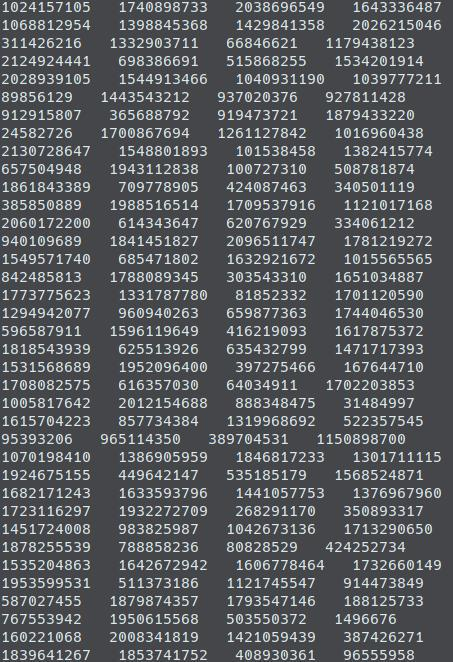
\includegraphics[width=0.4\textwidth]{1.jpg} }}
    \qquad
	\subfloat[]{{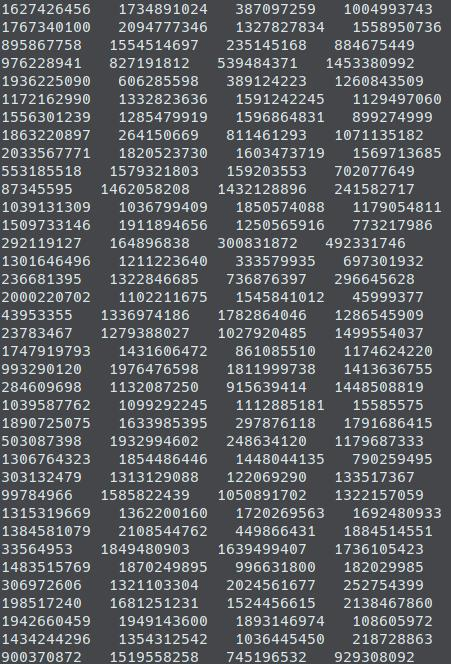
\includegraphics[width=0.4\textwidth]{5.jpg} }}
	\caption{}
	\label{p:91}
\end{figure}
\begin{figure}[H]
    \centering
	\subfloat[]{{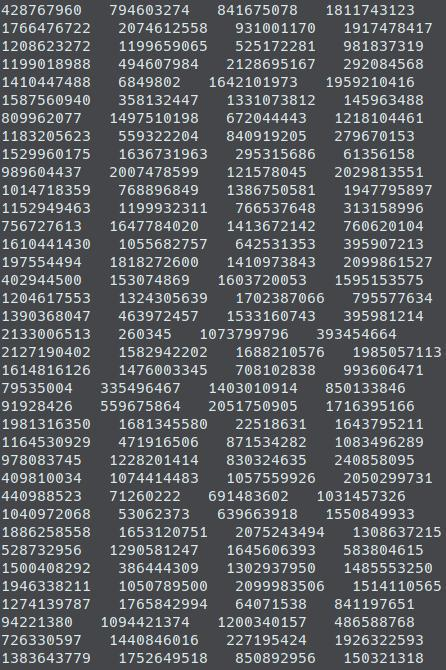
\includegraphics[width=0.4\textwidth]{3.jpg} }}
    \qquad
	\subfloat[]{{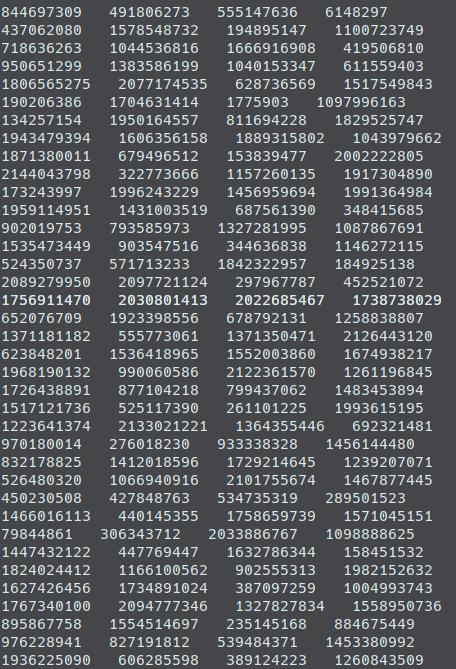
\includegraphics[width=0.4\textwidth]{4.jpg} }}
	\caption{}
	\label{p:92}
\end{figure}
\begin{figure}[H]
    \centering
	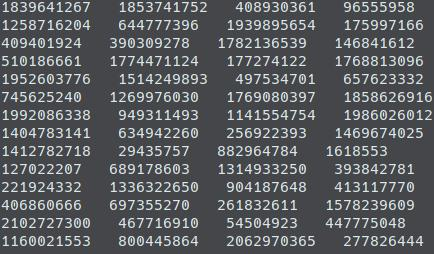
\includegraphics[width=0.5\textwidth]{6.jpg}
	\caption{}
	\label{p:93}
\end{figure}
\newpage
ЛКМ для генерації сотні чисел показані на рис \ref{p:94}:
\begin{figure}[H]
    \centering
	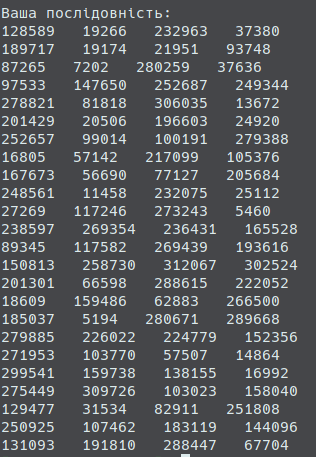
\includegraphics[width=0.5\textwidth]{2.png}
	\caption{}
	\label{p:94}
\end{figure}
\end{large}
\end{document}